\section{Theorie}
\label{sec:Theorie}
Stabile Isotope von Elementen weisen eine charakteristische Zusammensetzung ihrer Kerne aus Protonen und Neutronen auf, und werden bei Abweichungen von dieser instabil.
Dabei sind zumeist $20-50 \si{\percent}$ mehr Neutronen als Protonen vorhanden. Ein Maß für die Zerfallswahrscheinlichkeit verschiedener Isotope beziehungsweise Elemente ist
die Halbwertszeit $T$, welche die Zeit angibt bei welcher sich die Anzahl $N$ der Kerne halbiert hat. Zur Herstellung eines instabilen Isotopes kann die Aktivierung mit Neutronen
dienen. Dabei werden freie Neutronen durch Beschuss von Beryllium mit $\alpha$-Teilchen erzeugt. Da die Wahrscheinlichkeit für eine Aktivierung des Kernes durch ein freies Neutron
stark vom Wirkungsquerschnitt $\sigma$ abhängt, und dieser wiederum für langsamere Neutronen größer wird, werden die freien Neutronen nach ihrer Erzeugung verlangsamt.
Dazu dient eine Schicht aus Paraffin, in welcher die Neutronen durch elastische Stöße mit den Wasserstoffkernen, welche eine ähnliche Masse wie die Neutronen haben und deshalb
einen großen Energieübertrag ermöglichen, Energie, und somit Geschwindigkeit, verlieren.
Fängt der Kern ein Neutron ein, wird dessen Energie aufgrund der starken Wechselwirkung auf alle Nukleonen des Kerns verteilt, welche in Folge dessen auf höhere Energieniveaus wechseln.
Der nun enstandene Zwischenkern gibt Energie in Form eines $\gamma$-Quants ab, da er nicht in der Lage ist ein Nukleon abzustoßen. Der enstandene Kern ist je nach
Ausgangsmaterial nun instabil, da er ein Neutron mehr als ein stabiles Isotop enthält. Durch Umwandlung eines Neutrons in ein Proton unter Emission von $\beta$-Strahlung und eines Antineutrinos wird der
Kern nun wieder stabil. Zur quantitativen Beschreibung einer größeren Menge instabiler Kerne dient das Zerfallsgesetz:
\begin{equation}
  N(t)= N_0 e^{- \lambda t}
  \label{eqn:Zerfallsgesetz}
\end{equation}
mit der Zerfallskonstate $\lambda$ und der Zeit $t$. Über dieses lässt sich nun auch die Halbwertszeit bestimmen:
\begin{equation}
  T=\frac{\ln(2)}{\lambda}.
  \label{eqn:Halbwertszeit}
\end{equation}
Da zur Bestimmung der Zerfallskonstate und damit der Halbwertszeit das experimentell schwer zu messende $N(t)$ benötigt wird, wird unter Einführung einer festen Zeitdifferenz $\Delta t$
folgender Ausdruck hergeleitet:
\begin{equation}
  \ln(N_{\Delta t}(t)) =\ln(N_0 (1-e^{- \lambda \Delta t})) - \lambda t  .
  \label{eqn:Zerfallskonstante}
\end{equation}
Dies gilt für den Zerfall eines instabilen Isotops. Da aber zum Beispiel Silber in seiner natürlichen Form aus zwei Isotopen besteht, treten nach der Aktivierung zwei Zerfallsprozesse
auf. Ähnliches gilt für Rhodium, welches zwar nur aus einem Isotop besteht, jedoch durch die Aktivierung in zwei verschieden wahrscheinliche Zustände umgewandelt wird.
Liegt ein solcher Fall vor, kann durch Ausnutzen der verschieden schnellen Zerfälle der zwei instabilen Isotope trotzdem die jeweilige Halbwertszeit ermittelt werden. Dazu wird ein Zeitpunkt
in der Zerfallskurve gewählt an welchem der schnellere Zerfall so weit fortgeschritten ist, dass fast nur noch der langsamere Zerfall stattfindet. So lässt sich eine Kurve für den
langsamen Zerfall optimieren welche vom Gesamtzerfall subtrahiert wird und so den schnelleren Zerfall sichtbar macht. Dies ist in Abbildung \ref{fig:2Isotope} dargestellt.
\FloatBarrier
\begin{figure}
  \centering
  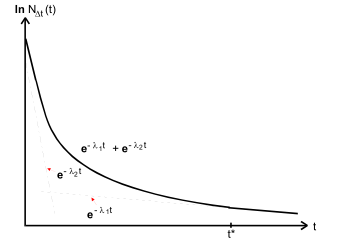
\includegraphics{images/2Isotope.png}
  \caption{Beispiel für überlagerte Zerfallskurven zweier Isotope.\cite{sample}}
  \label{fig:2Isotope}
\end{figure}
\FloatBarrier
